\chapter{Physical Layer}

\section{Network Architecture}
A \keyword{network architect} designs the network (topology, standards, connections, where to put cables). A \keyword{network engineer} installs the equipment to setup the network.

\termdef{Patch Panel/Socket Panel}{
    \begin{center}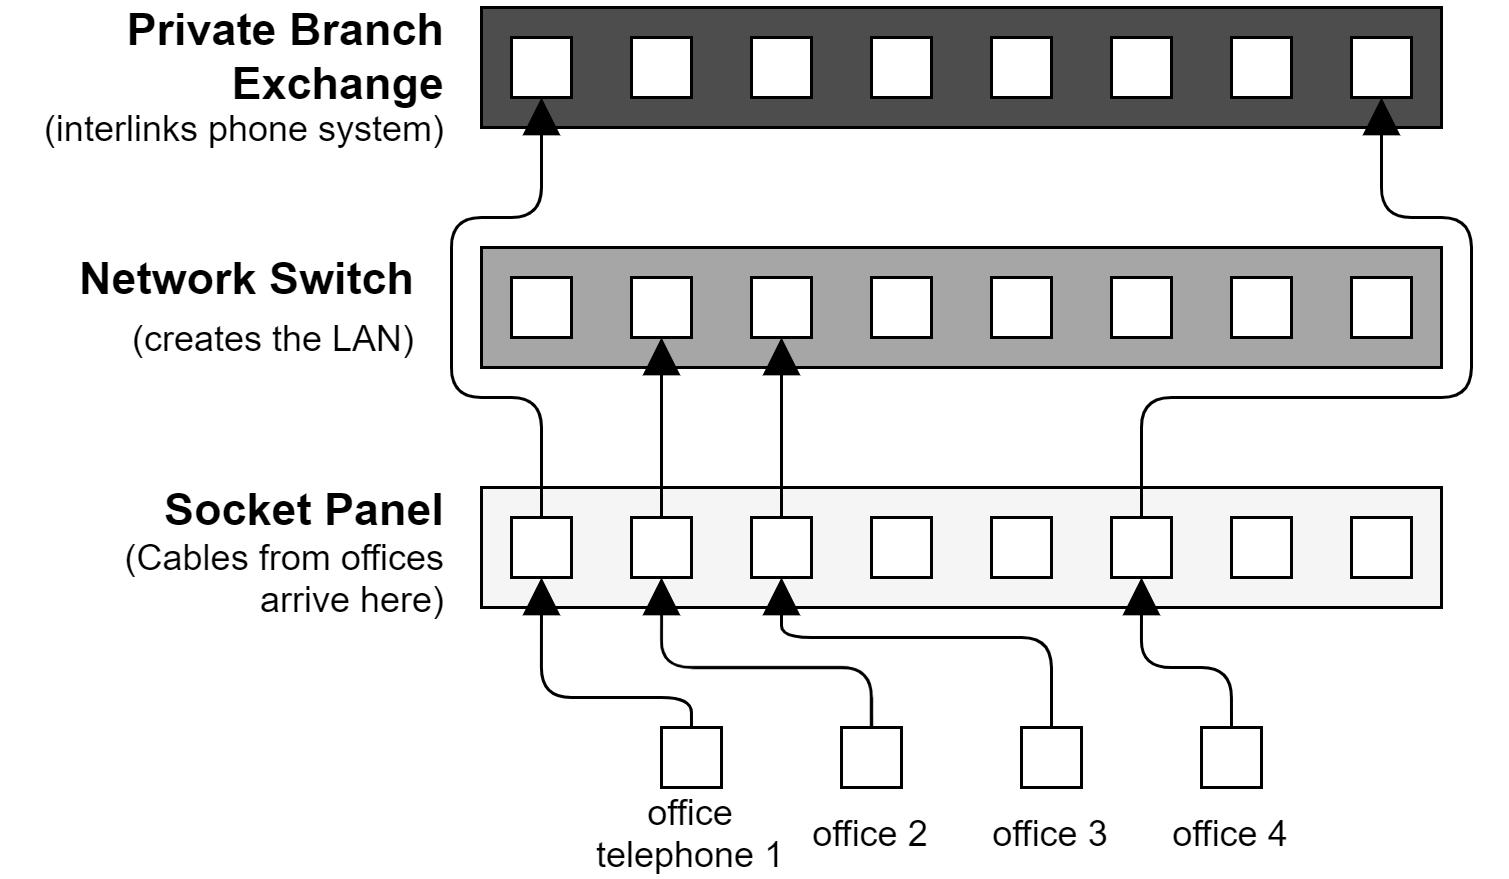
\includegraphics[width=0.9\textwidth]{physical_layer/images/patch panel}\end{center}
    The \keyword{PBX} (\keyword{Private Branch Exchange}) is used for phones, however if the phone system is \keyword{IP} based, a separate \keyword{PBX} is not needed.
}

\section{Wired Transmission}
\termdef{Unshielded Twisted Pair (UTP)}{
    Two wires twisted together.
    \compitem{
        \item Cheap \& easy to mass-produce.
        \item Twisting reduces interference and crosstalk between cables.
        \item Used in telephone systems.
    }
    \begin{center}
        \begin{tabular}{l l l}
            \textbf{Type} & \textbf{Speed} & \textbf{Description}                                   \\
            CAT1          & $1 Mbps$       & Voice grade for POTS (plain old telephone service).    \\
            CAT5          & $100 Mbps$     & 10Base-T Ethernet Cables and 100Base-TX Fast Ethernet. \\
            CAT6          & $1,000 Mbps$   & 1000Base-T Gigabit Ethernet.                           \\
        \end{tabular}
    \end{center}
}
\termdef{Coaxial Cable}{
    Conductors placed concentrically (one inside the other), separated by an insulator.
    \begin{center}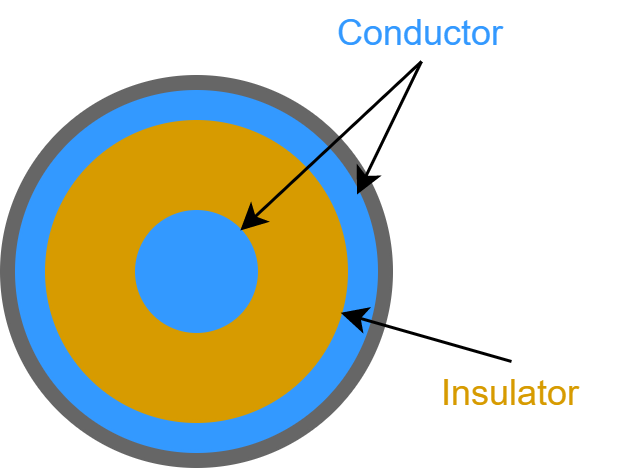
\includegraphics[width=0.4\textwidth]{physical_layer/images/coaxial cable}\end{center}
    \compitem{
        \item Good sheilding, electromagnetic field mainly between inner and outer conductor.
        \item Large bandwidth from high range of frequencies.
        \item Higher cost per meter (hence \keyword{UTP} is more popular for common consumption).
    }
}
\termdef{Optical Fibre}{
    Transmits data using light and refraction (explained well \href{https://www.youtube.com/watch?v=F6OA_jvnwus}{here}).
    \compitem{
        \item Single optical fibre is 2 - 125 micrometers in diameter.
        \item \keyword{Attenuation} (signal loss) is low, so can be used for long distances.
        \item Very high bandwidth.
    }
    \begin{tabular}{l l l}
        \textbf{Year} & \textbf{Speed} & \textbf{Organisation}                                                  \\
        2011          & $26 \ Tbps$    & Karlsruhe Institute of Technology                                      \\
        2014          & $43 \ Tbps$    & Technical University of Denmark                                        \\
        2014          & $255 \ Tbps$   & Eindhoven University of Technology and University of Central Florida   \\
        2021          & $319 \ Tbps$   & Japan National Institute of Information \& Communications Technology   \\
        2021          & $1000 \ Tbps$  & {Japan National Institute of Information \& Communications Technology} \\
    \end{tabular}
}
\begin{center}
    \begin{tabular}{l l l l l}
                                & \textbf{Freq Range} & \textbf{Attenuation}      & \textbf{Delay}   & \textbf{Repeater Spacing} \\
        \keyword{UTP}           & $0-1 \ MHz$         & $0.7 \ dB/km$ @ $1 \ KHz$ & $5 \ \mu s /km$  & $2 \ km$                  \\
        \keyword{Coaxial Cable} & $0-500 \ MHz$       & $7 \ dB/km$ @ $10 \ MHz$  & $4 \ \mu s / km$ & $1-9 \ km$                \\
        \keyword{Optical Fibre} & $186-370 \ THz$     & $0.2-0.5 \ dB/km$         & $5 \ \mu s / km$ & $40 \ km$                 \\
    \end{tabular}
\end{center}

\section{Wireless Transmission}
Done using electromagnetic radiation (typically radio).
\compitem{
    \item No need for wires (expensive \& take time to install).
    \item Bidirectional communication by default.
    \item Typically broadcast (e.g all/most recievers can see transmissions) (works with many stations).
    \item Inverse square law - signal strength reduces with range.
    \item Environment degrades signal (interference, obstruction, reflection of signal).
}
\sidenote{Wave Types}{
    For more look at chapter 3 of \href{https://upload.wikimedia.org/wikipedia/commons/d/d8/Communication_Systems.pdf}{Communication Systems}.
}

\section{Information Representation}
\twosplit{
    \termdef{Digital}{
        Discrete information, represented by a finite number of states.
        \\
        \\ e.g $0$ and $1$ for binary.
    }
}{
    \termdef{Analogue}{
        Continuous information, represented by changes in some physical state.
        \\
        \\ e.g light intensity, voltage.
    }
}
\termdef{Baud Rate (Bd)}{
    Symbol rate per second for a digital channel, where a symbol may represent more than 1 bit.
}

\termdef{Modem}{
    \begin{center}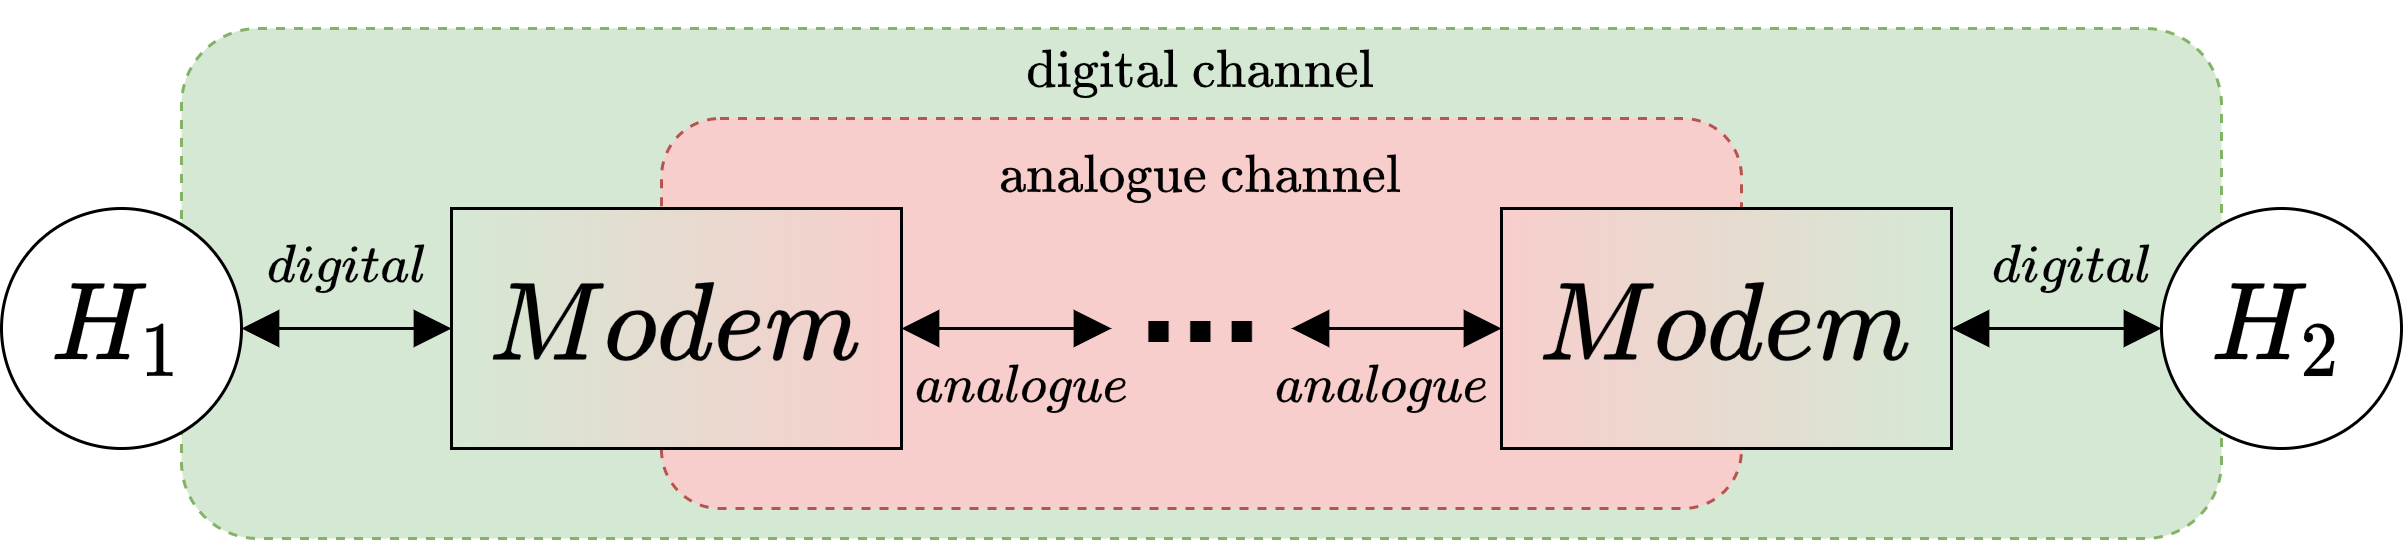
\includegraphics[width=0.9\textwidth]{physical_layer/images/digital analogue channels}\end{center}
    A \keyword{Modulator-Demodulator} implements a digital channel using an analogue channel.
    \begin{center}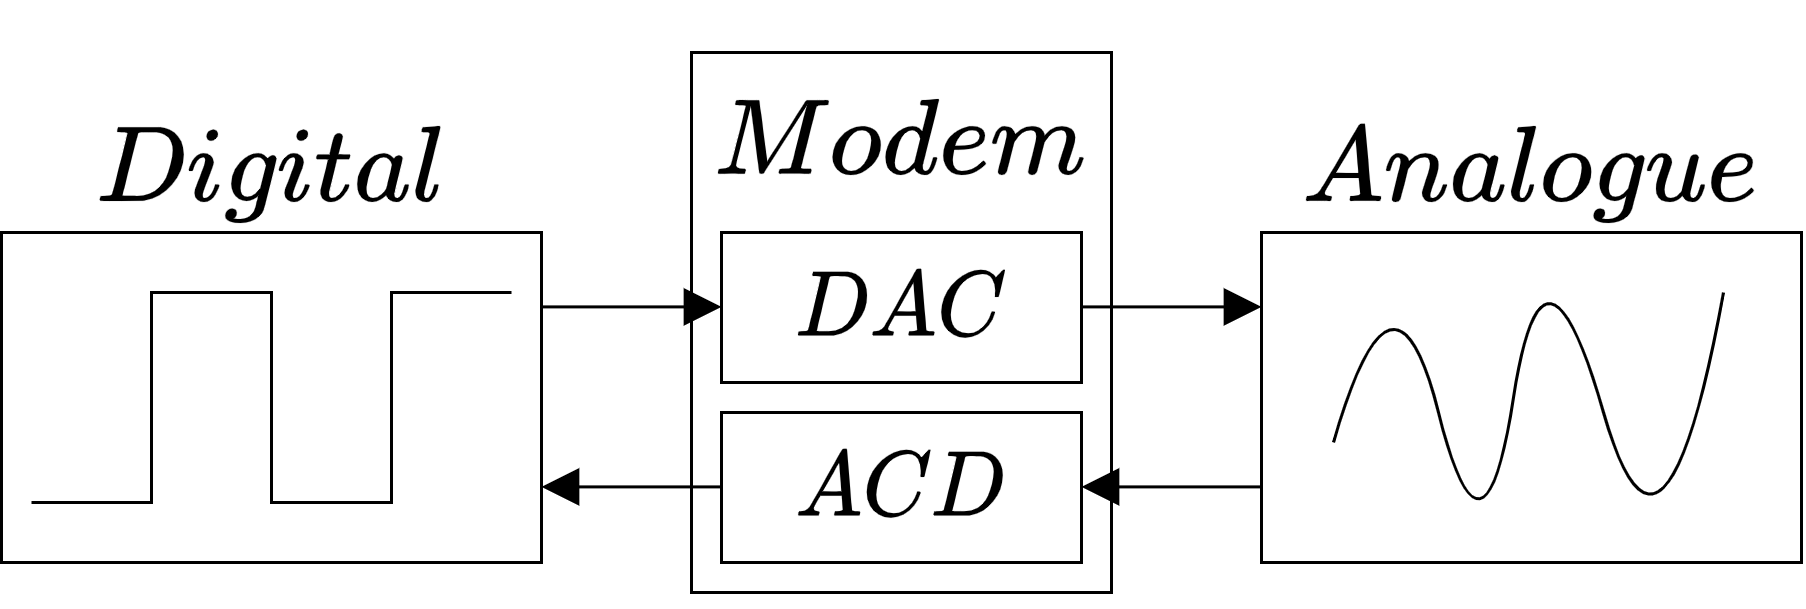
\includegraphics[width=0.7\textwidth]{physical_layer/images/modem}\end{center}
    \compitem{
        \item \keyword{DAC} $\to$ \keyword{Digital to Analogue Converter}
        \item \keyword{ADC} $\to$ \keyword{Analogue to Digital Converter}
    }
}

\termdef{Codec}{
    A \keyword{Coder-Decoder} implements an analogue channel using a digital channel.
}
\subsubsection{Waves}
\begin{center}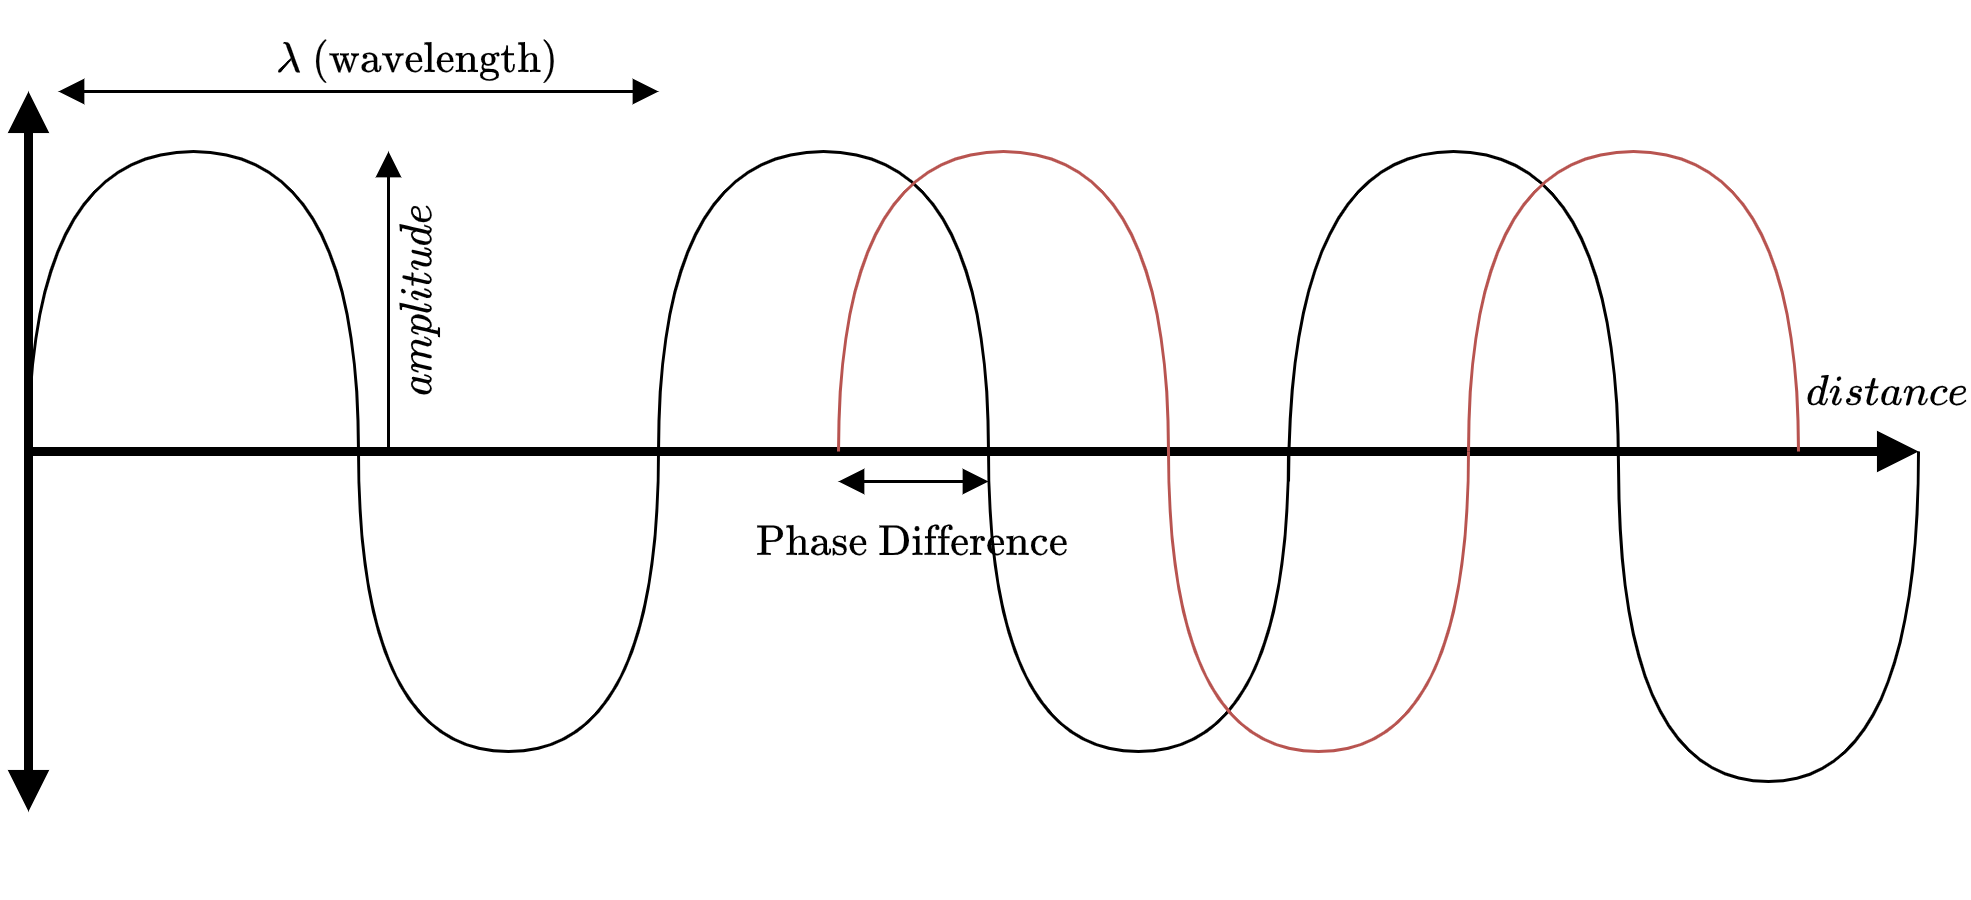
\includegraphics[width=0.8\textwidth]{physical_layer/images/waveform}\end{center}
\begin{center}
    \begin{tabular}{l c p{0.8\textwidth}}
        \keyword{Amplitude} &           & Maximum displacement/strength of the signal. \\
        \keyword{Wavlength} & $\lambda$ & Length of a single cycle.                    \\
        \keyword{period}    & $p$       & The time taken to complete a cycle.          \\
        \keyword{Frequency} & $f$       & The number of cycles per second.             \\
    \end{tabular}
\end{center}

\[\begin{split}
        p &= \cfrac{1}{f} \text{  (period and frequency)} \\
        wavespeed &= f \lambda \text{  (for radio waves} wavespeed = c = 3 \times 10^8 ms^{-1} \text{ )} \\
    \end{split}\]

\sidenote{Phase}{
    Given two waves of the same wavelength and speed/frequency, they may be offset by some distance.
    \\
    \\ The pahse difference can be considered as a distance, or fraction of a cycle. In the latter anglke units may be used (full cycle $= 360\deg = 2\pi$).
    \\
    \\ The maximum phase difference is $\pi$, where the waves are in opposite displacements for any given time during their cycle.
}
\section{Modulation}
A \keyword{modulation} scheme is used to change some information signal into one more suitable for transmission.
\begin{center}
    \begin{tabular}{l p{0.7\textwidth}}
        \keyword{Baseband Modulation}  & Transmit unmodified (dedicated line sending in full). \\
        \keyword{Broadband Modulation} & {
                Uses a basic carrier signal to encode information. The carrier signal has modifications added to encode information (e.g changing amplitude, frequency or phase).
        }                                                                                      \\
    \end{tabular}
\end{center}
\subsection{Amplitude Modulation / Amplitude Shift Keying (ASK)}
\begin{center}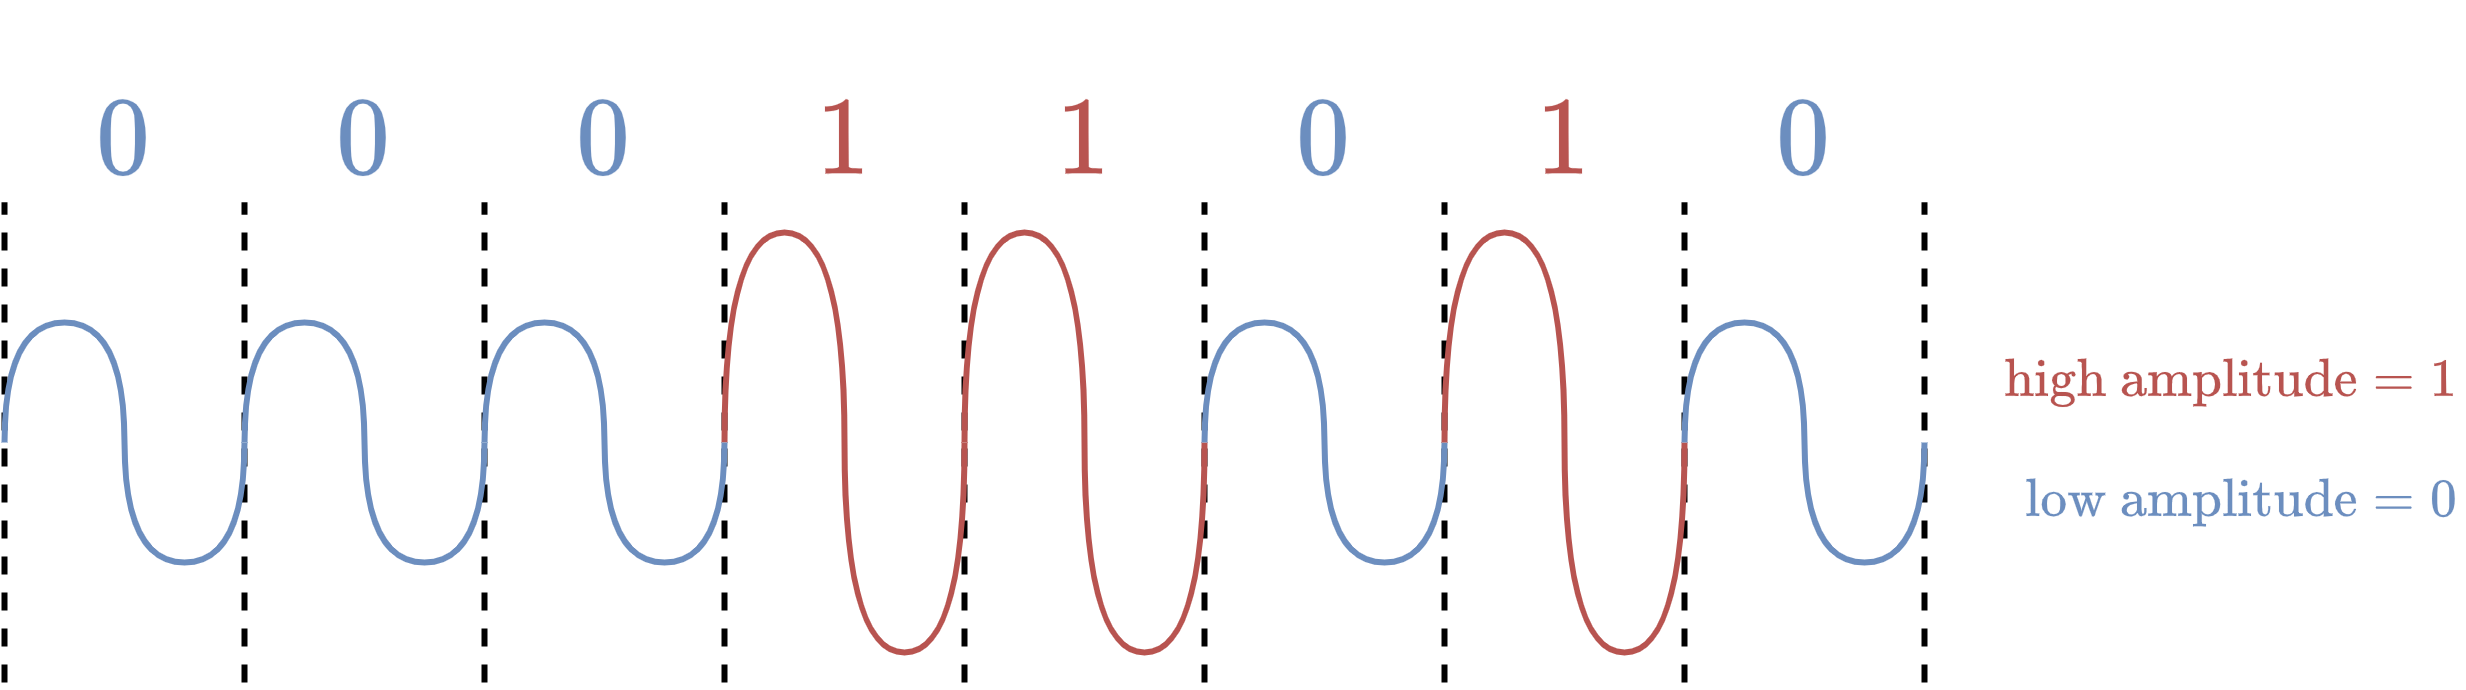
\includegraphics[width=0.9\textwidth]{physical_layer/images/amplitude modulation}\end{center}

\subsection{Frequency Modulation / Frequency Shift Keying (FSK)}
\begin{center}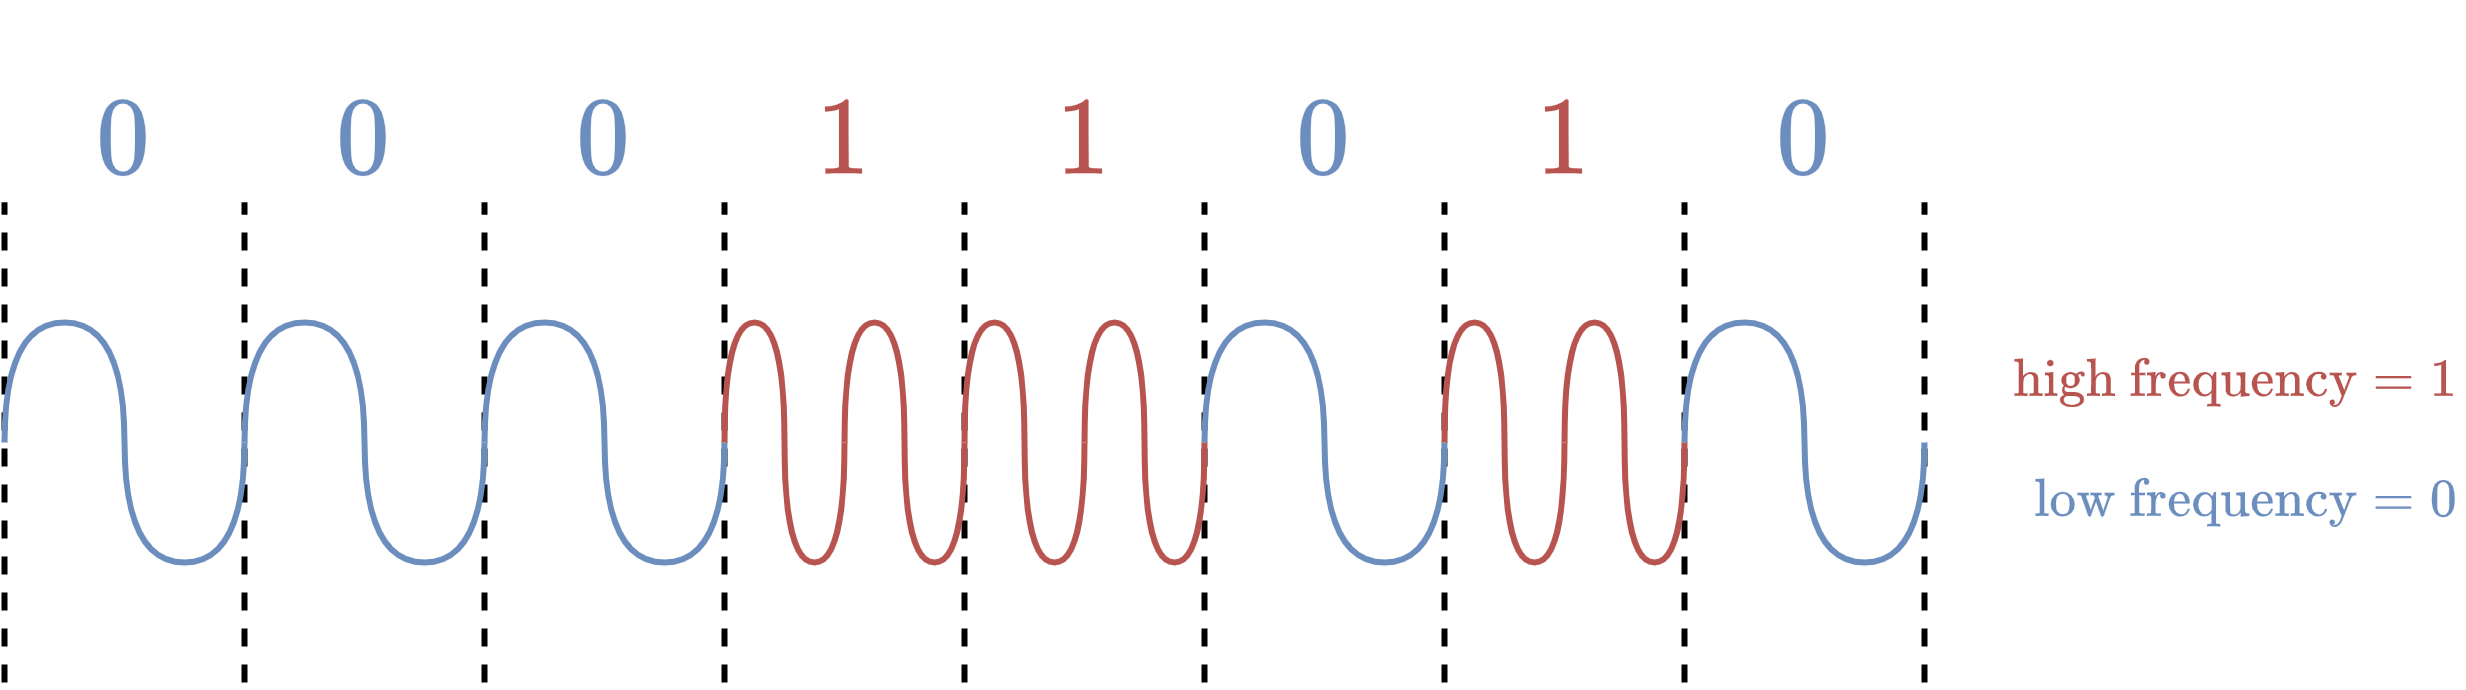
\includegraphics[width=0.9\textwidth]{physical_layer/images/frequency modulation}\end{center}

\subsection{Phase Modulation}
\begin{center}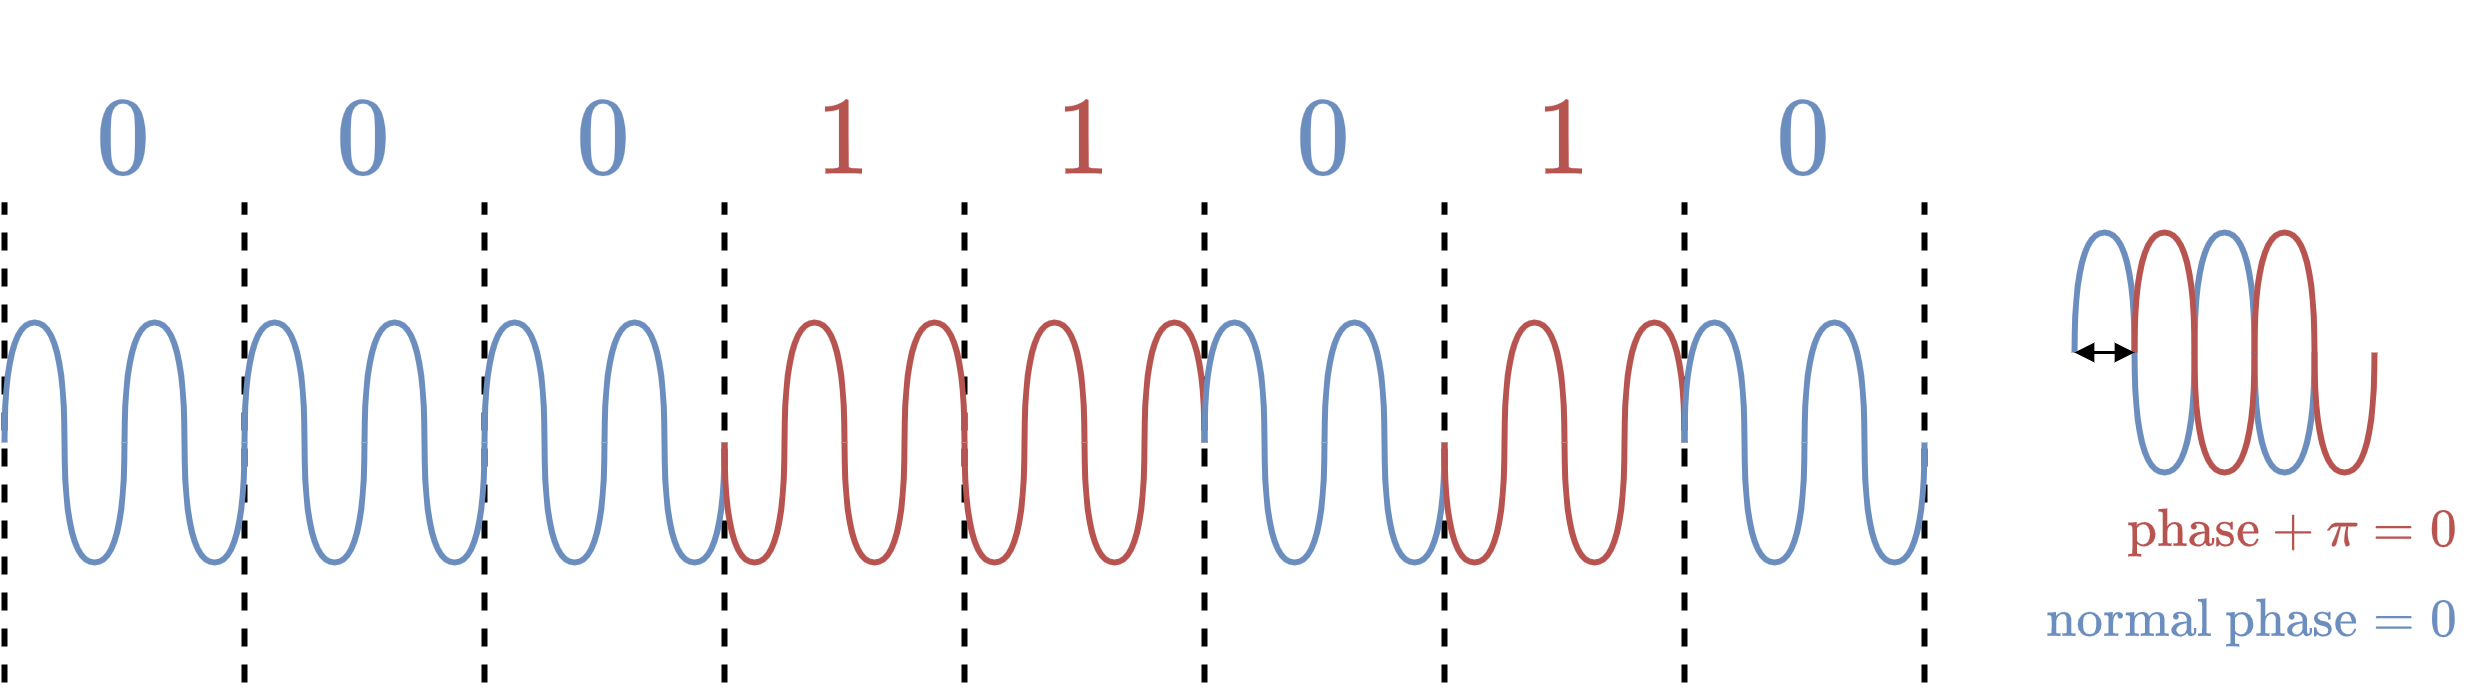
\includegraphics[width=0.9\textwidth]{physical_layer/images/phase modulation}\end{center}

\subsection{Better Modulation}
To improve the data rate we can transmit multiple bits per symbol (in modulation scheme).
\compitem{
    \item Use more phase differences, amplitudes.
    \item Use a combination of phase, amplitude to determine symbol.
}
For example we can use phase (interpreted as an angle) in combination with amplitude in a scheme such as \keyword{QAM}.
\begin{center}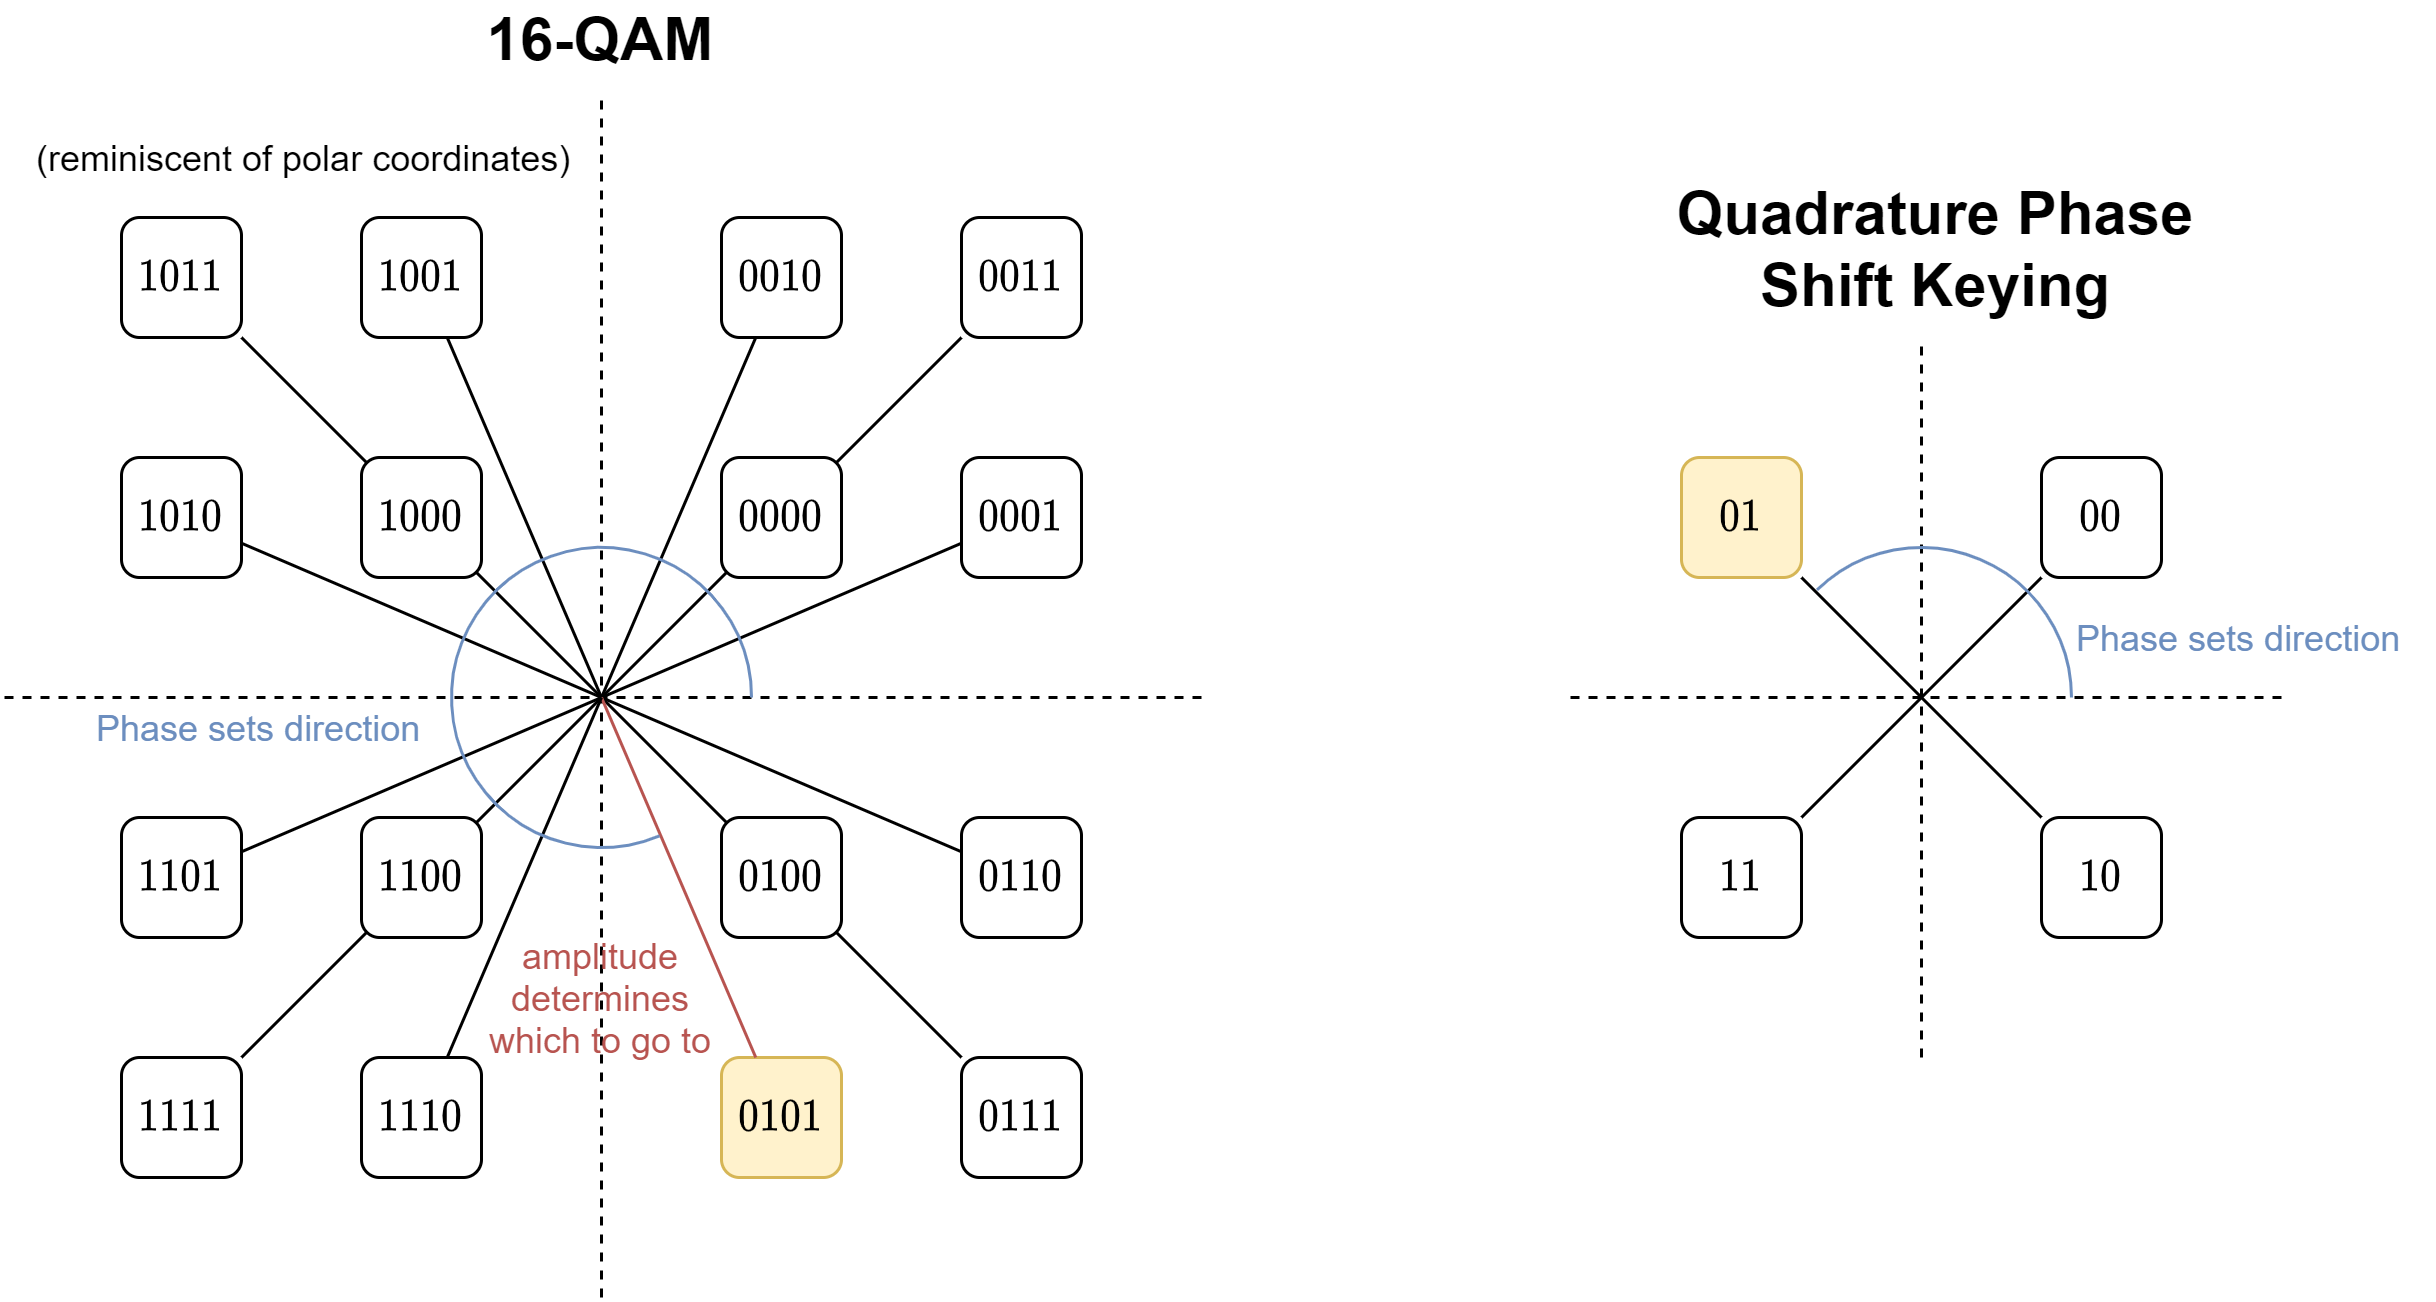
\includegraphics[width=0.9\textwidth]{physical_layer/images/quadrature phase shift keying}\end{center}

\subsection{Digital Subscriber Line (DSL)}
With the V.90 Modem Standard, using conventional phone lines to transfer data.
\compitem{
    \item Maximum $56,000 \ bps$ downstream (download) and $33,000$ upstream (upload)
    \item Limited as phone lines limited to $3,000 \ Hz$ bandwidth (human voice goes to $3,400 \ Hz$ and was originally developed only for voice communication).
    \item Anything outside that range is filtered out as noise.
}
By removing the limitation (by removing the bandwidth filter) \keyword{DSL} allows for more bandwidth and hence a higher data rate.
\\
\\ However noise now becomes a limiting factor.

\subsection{Asymmetric Digital Subscriber Line (ADSL)}
\begin{center}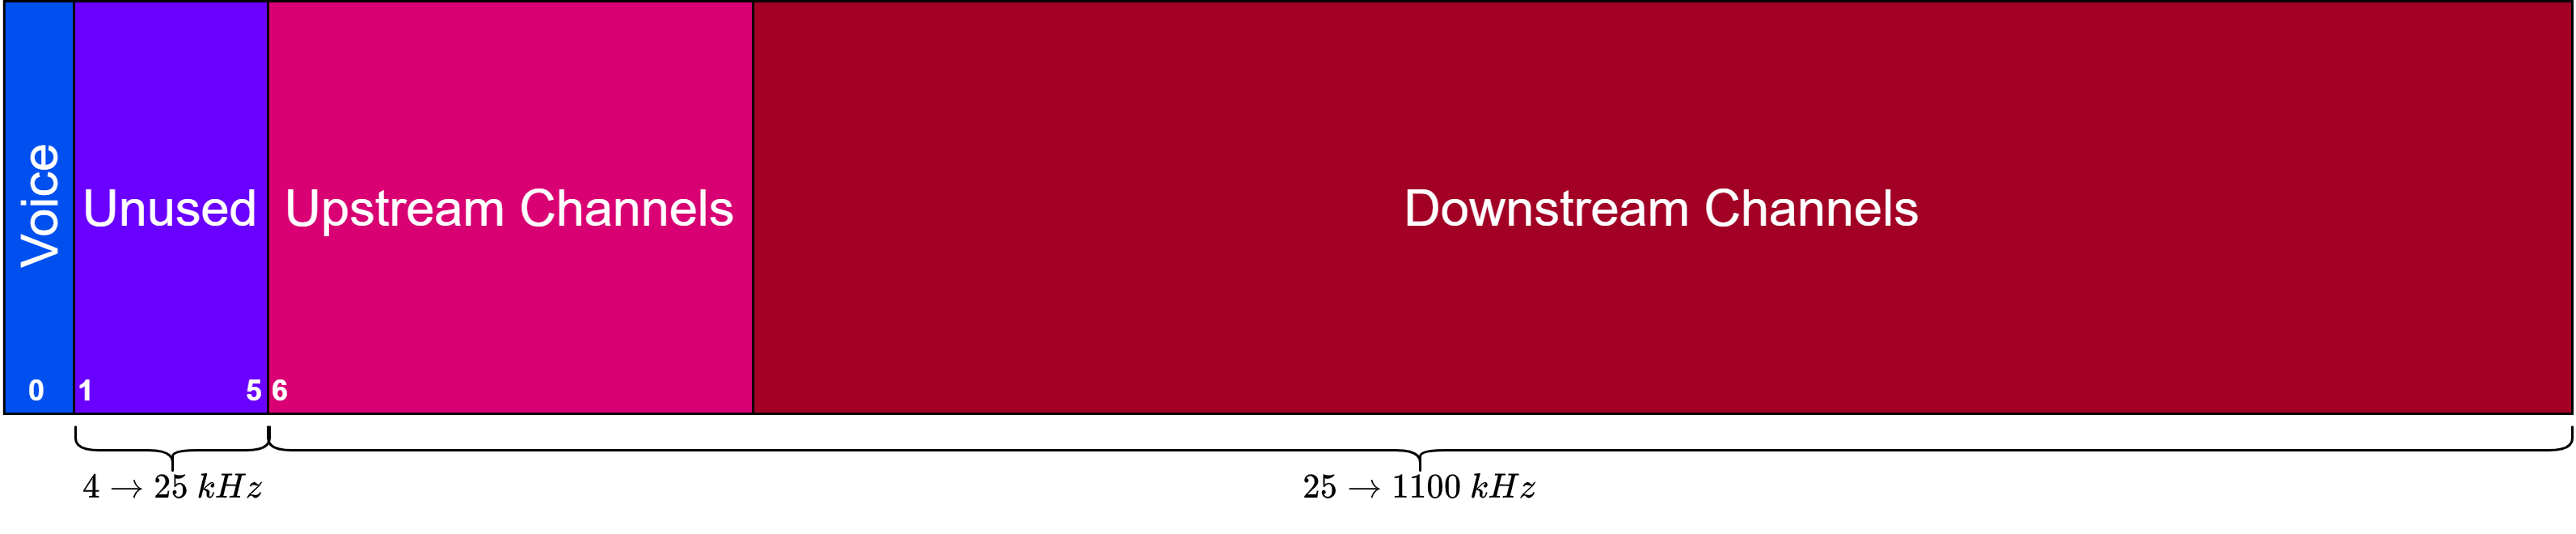
\includegraphics[width=0.9\textwidth]{physical_layer/images/ADSL}\end{center}
\compitem{
    \item $1.1 \ MHz$ of bandwidth divided into $256$ $4000 \ Hz$ channels.
    \item Channels $1 \to 5$ ($4 \to 25 \ kHz$) are unused to avoid interference between voice and data channels.
    \item More channels are allocated to download than upload as download used more heavily.
    \item Voice is cahnnel $0$ ($0 \to 4 \ kHz$)
    \item V.24 modulation uses 224 downstream channels ($13.44 \ Mbps$)
    \item A \keyword{ADSL Splitter} separates the voice band from data.
    \item An \keyword{ADSL modem} performs modulation.
}

\keyword{DSL Access Multiplexer} (\keyword{DSLAM}) (typically owned by the \keyword{ISP}) connects local telephone cables to the \keyword{ISP}
\begin{center}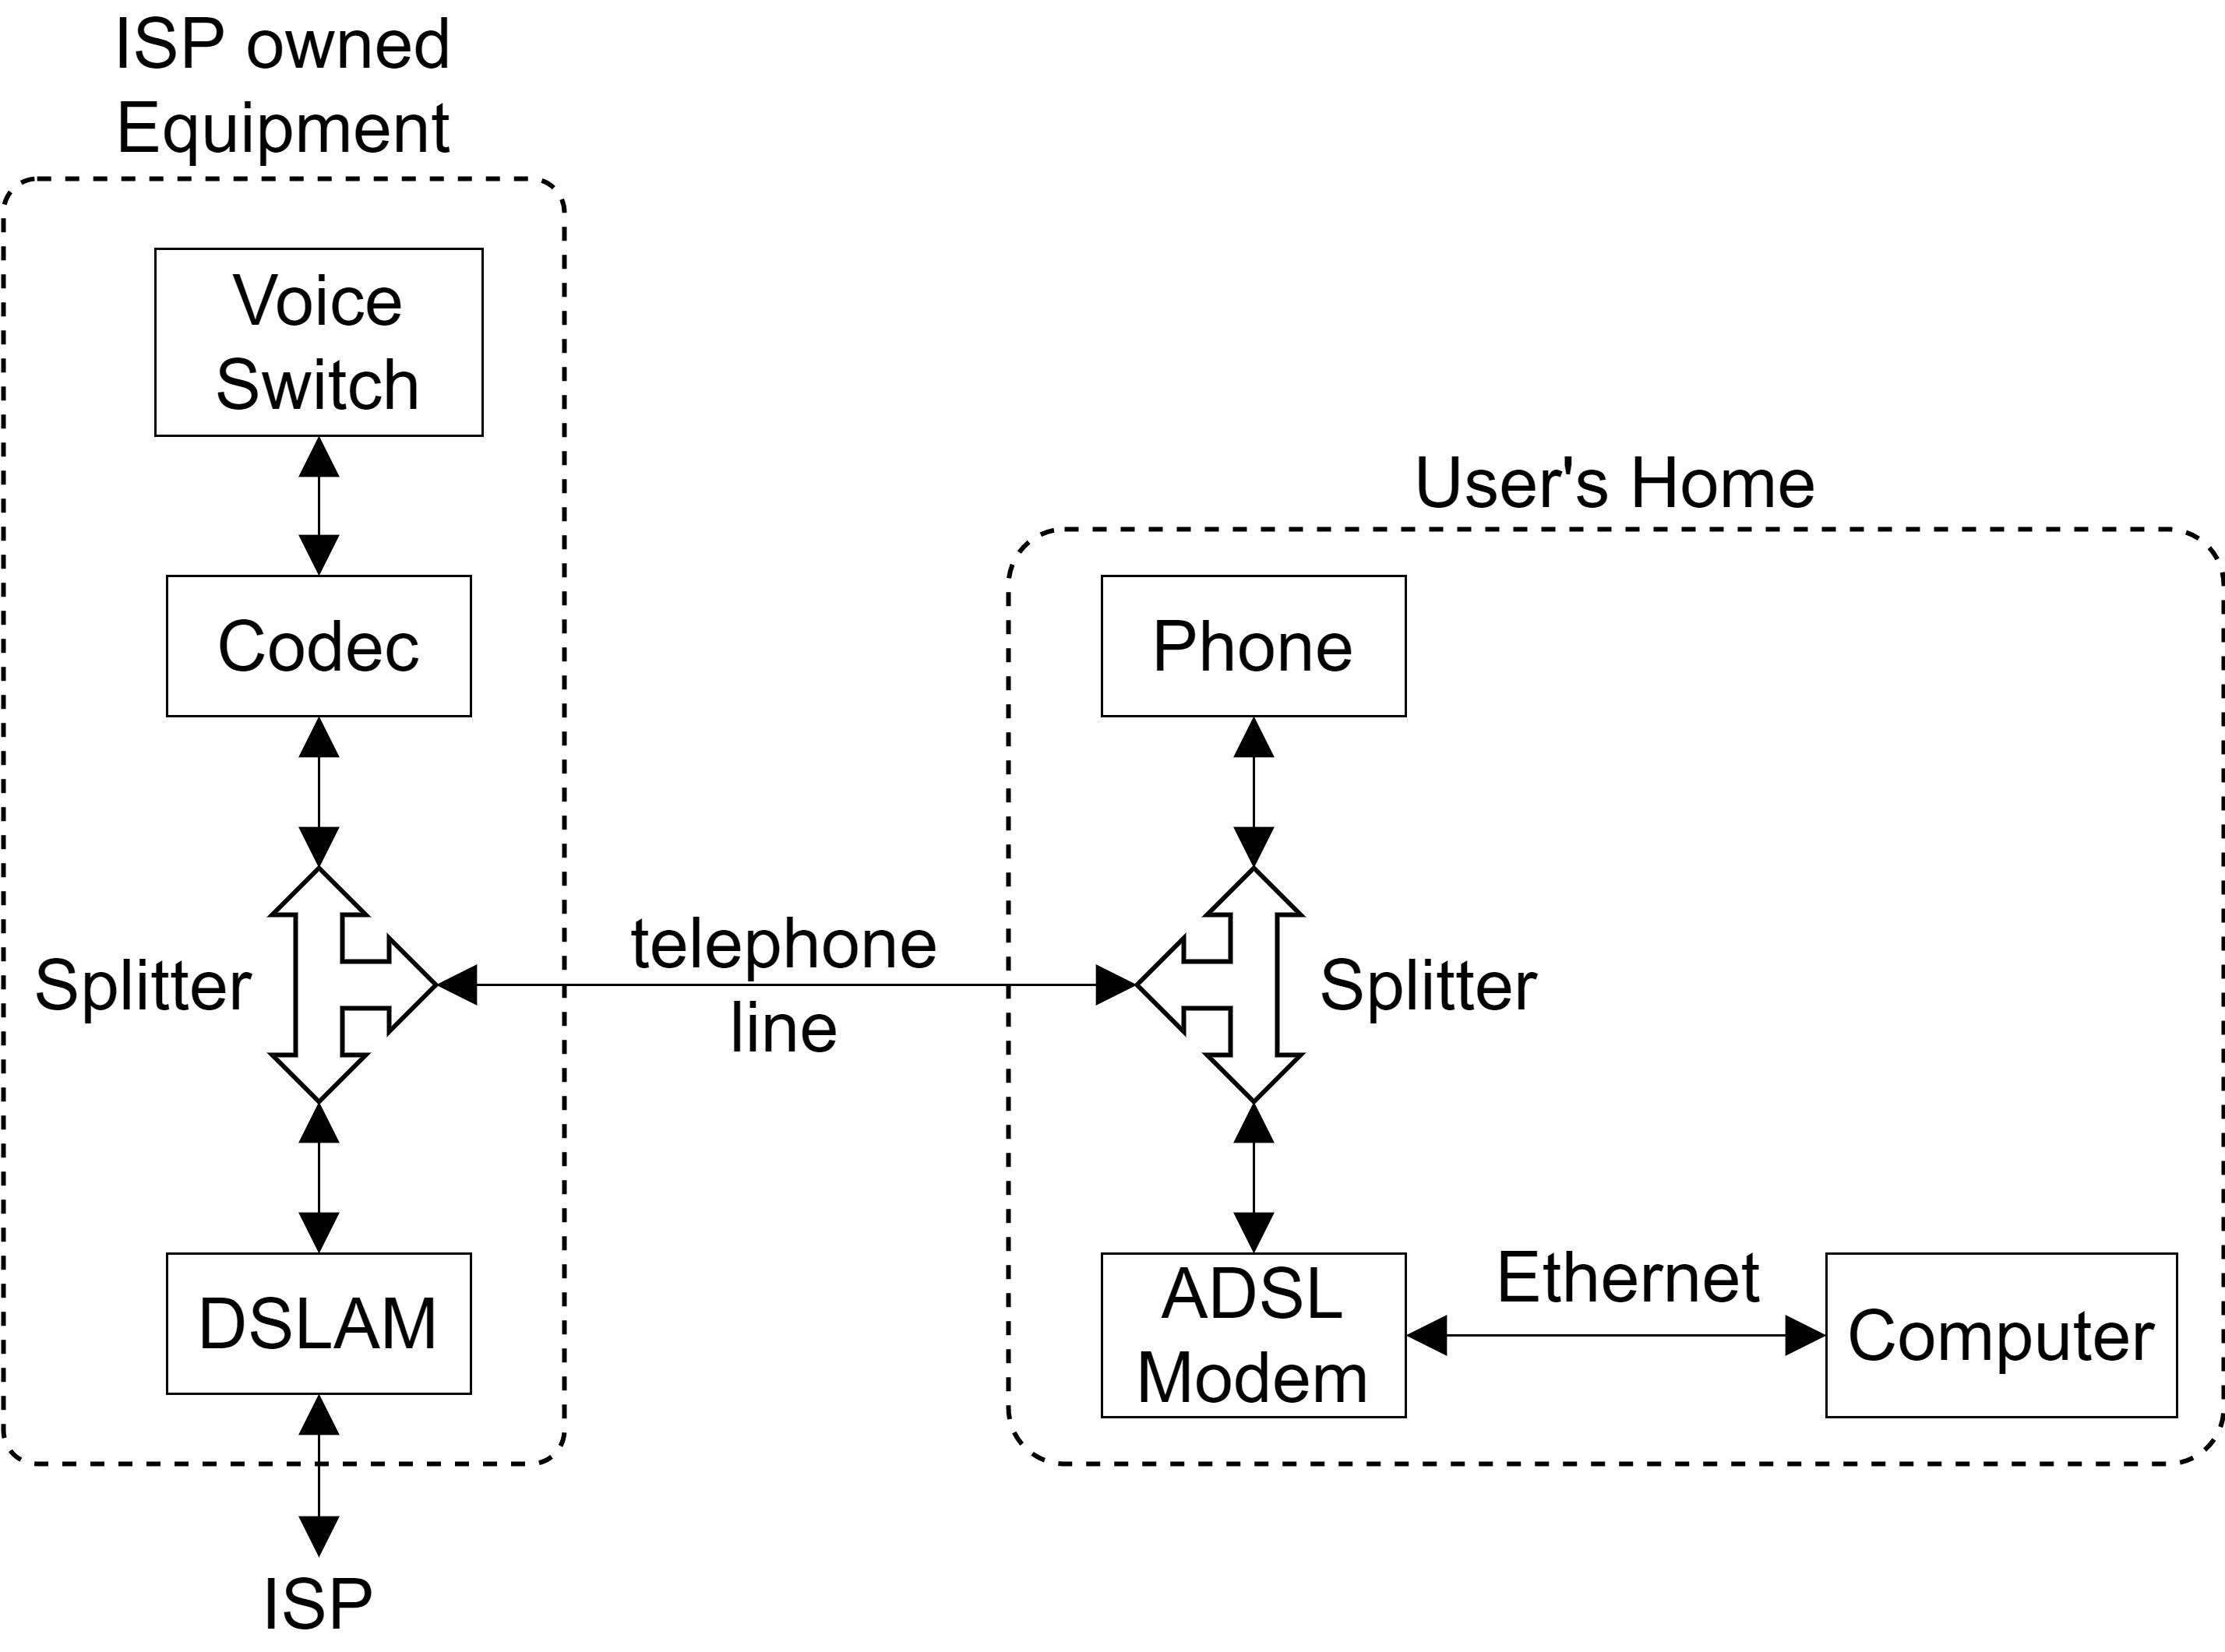
\includegraphics[width=0.9\textwidth]{physical_layer/images/DSL Access Multiplexer}\end{center}

\subsection{DSL Advancement}
\begin{tabular}{l l l l}
    \keyword{ADSL2}  & $12 \ Mbps$  & $2.2 \ MHz$                          \\
    \keyword{ADSL2+} & $12 \ Mbps$  & $2.2 \ MHz$ & More bits per symbol   \\
    \keyword{VDSL}   & $52 \ Mbps$  & $12 \ MHz$  & Very-high-bit-rate DSL \\
    \keyword{VDSL2}  & $200 \ Mbps$ & $30 \ MHz$  & Currently popular      \\
\end{tabular}
\begin{center}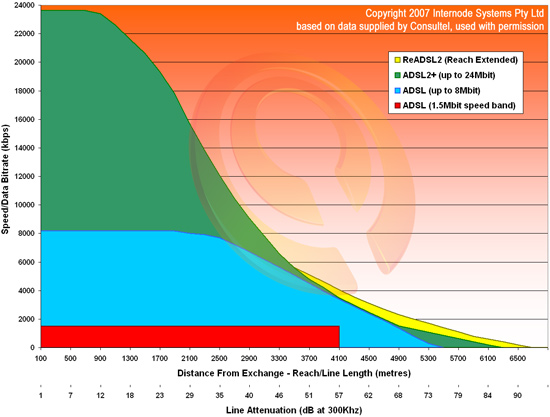
\includegraphics[width=0.7\textwidth]{physical_layer/images/Internode DSL}\end{center}

\section{Network Simulation}
Network simulation is used to design networks cheaply.
\\
\\ Different simulators provide different features:
\compitem{
    \bullpara{Cisco Packet Tracer}{Strong adacemic backing}
    \bullpara{gns3}{Strong, open community backing}
    \bullpara{OPNET}{Professional use, quite technical}
}

Cisco packet Tracer allows code to be run inside the simulation:
\compitem{
    \item Cisco IOS commands (Cisco's proprietary Operating System)
    \item Terminal commands inside applications on Desktop/Laptops
    \item Web documents (through server's http service)
    \item Python \& Javascript
    \item MQTT (Message Queue Telemetry Transport) (a lightweight machine-to-machine Publisher/Subscriber messaging protocol)
    \item
}

\section{Network Programming}

\subsection{Simple Echo}
\compenum{
    \item Run server, waiting for connections on a user-defined port.
    \item Client connects to the port.
    \item Server listens for input from the client.
    \item User types into client, client sends message to server.
    \item Server echos recieved data back to client.
    \item Client disconnects.
    \item Server closes.
}
\codelist{Java}{physical_layer/code/EchoClient.java}
\codelist{Java}{physical_layer/code/EchoServer.java}

\subsection{Concurrent Executor}
We can use a thread pool to handle running tasks for many clients connecting, and sending input.
\codelist{Java}{physical_layer/code/ConcurrentServer.java}
\sidenote{Oracle Guides}{
    The guides these examples were based on can be found \href{https://www.oracle.com/webfolder/technetwork/tutorials/obe/java/SocketProgramming/SocketProgram.html}{here}.
}

